% Editable, self-contained LaTeX report. Compiler: pdfLaTeX.
% The cover, section order and table/figure style closely follow the supplied
% Group 065/083 reference. Implementation details and data describe Group 097/112.
% All charts are native PGFPlots: no external image or table files are required.
\documentclass[11pt,a4paper]{article}
\usepackage[top=25mm,bottom=22mm,left=25mm,right=25mm,footskip=11mm]{geometry}
\usepackage[T1]{fontenc}
\usepackage{courier}
\usepackage[scaled=0.95]{helvet}
\renewcommand{\familydefault}{\sfdefault}
\usepackage{amsmath,microtype,array,tabularx}
\usepackage[table]{xcolor}
\usepackage{titlesec,fancyhdr,enumitem}
\usepackage[obeyspaces]{url}
\usepackage[hidelinks]{hyperref}
\usepackage{pgfplots}
\pgfplotsset{compat=1.18}
\definecolor{heading}{HTML}{203864}
\definecolor{tablehead}{HTML}{D9E2F3}
\definecolor{gridline}{HTML}{A6AFC0}
\definecolor{muted}{HTML}{666666}
\definecolor{barblue}{HTML}{315F8A}
\definecolor{barorange}{HTML}{D88B32}
\definecolor{bodytext}{HTML}{222222}
\color{bodytext}
\setlength{\parindent}{0pt}
\setlength{\parskip}{6pt}
\linespread{1.08}
\raggedbottom
\setlist[itemize]{leftmargin=16pt,itemsep=4pt,topsep=4pt}
\titleformat{\section}{\color{heading}\large\bfseries}{\thesection.}{0.45em}{}
\titleformat{\subsection}{\color{heading}\normalsize\bfseries}{\thesubsection}{0.45em}{}
\titleformat{\subsubsection}{\color{heading}\normalsize\bfseries}{\thesubsubsection}{0.45em}{}
\titlespacing*{\section}{0pt}{12pt}{5pt}
\titlespacing*{\subsection}{0pt}{9pt}{4pt}
\titlespacing*{\subsubsection}{0pt}{7pt}{3pt}
\newcolumntype{P}[1]{>{\raggedright\arraybackslash}p{#1}}
\newcolumntype{Y}{>{\raggedright\arraybackslash}X}
\newcolumntype{C}{>{\centering\arraybackslash}X}
\newcolumntype{R}{>{\raggedleft\arraybackslash}X}
\newcommand{\code}[1]{\nolinkurl{#1}}
\newcommand{\tablecaption}[1]{\refstepcounter{table}\par\smallskip{\small\bfseries\color{heading}Table \thetable. #1}\par\smallskip}
\newcommand{\figurecaption}[1]{\refstepcounter{figure}\par\smallskip{\centering\small\itshape\color{muted}Figure \thefigure. #1\par}\smallskip}
\newcommand{\hdr}{\rowcolor{tablehead}\bfseries}
\newcommand{\rowend}{\\\hline}
\newcommand{\nextpage}{\newpage}
\arrayrulecolor{gridline}
\setlength{\tabcolsep}{6pt}
\renewcommand{\arraystretch}{1.3}
\pgfplotsset{reportaxis/.style={width=0.95\linewidth,height=56mm,font=\small,axis lines*=left,tick align=outside,ymin=0,ymajorgrids=false,enlarge x limits=0.2,xtick=data,scaled y ticks=false,legend style={draw=none,font=\footnotesize},title style={font=\small},label style={font=\small},tick label style={font=\small}}}

% ---------------- EDIT GROUP DETAILS HERE ----------------
\newcommand{\GroupOne}{097}
\newcommand{\GroupTwo}{112}
\newcommand{\MemberOne}{Aryan Dalsaniya}
\newcommand{\RollOne}{202401405}
\newcommand{\MemberTwo}{Harshil Shah}
\newcommand{\RollTwo}{202401468}
\newcommand{\MemberThree}{Dhvanit Shah}
\newcommand{\RollThree}{202401467}
\newcommand{\MemberFour}{Dwij Patel}
\newcommand{\RollFour}{202401418}
\newcommand{\MemberFive}{Tanishq Shah}
\newcommand{\RollFive}{202401474}
\newcommand{\MemberSix}{Niranjan Panchal}
\newcommand{\RollSix}{202401441}
% These roles are proposed; confirm actual contributions before submission.
\newcommand{\RoleOne}{Part I single-threaded server, topic discovery and integration.}
\newcommand{\RoleTwo}{Client protocol, file reception and integrity checks.}
\newcommand{\RoleThree}{Part I multithreaded server and concurrency experiments.}
\newcommand{\RoleFour}{Part II Case 1: fault injection and restart-from-beginning recovery.}
\newcommand{\RoleFive}{Part II Case 2: session management, checkpoints and automated tests.}
\newcommand{\RoleSix}{Part II Case 2 Enhanced: parallel connections and performance analysis.}
\hypersetup{pdftitle={Final Report: Fault Tolerant Topic-based File Distribution Service},pdfauthor={Groups 097 and 112}}
\pagestyle{fancy}\fancyhf{}
\renewcommand{\headrulewidth}{0pt}\renewcommand{\footrulewidth}{0pt}
\fancyfoot[C]{\footnotesize\color{muted}Group \GroupOne\ and \GroupTwo\enspace |\enspace IT305 Socket Programming Project\enspace |\enspace Page \thepage}

\begin{document}
% ======================== PAGE 1 ========================
\thispagestyle{empty}
\begin{center}
\vspace*{2mm}
{\large\bfseries\color{muted}DHIRUBHAI AMBANI UNIVERSITY\par}
\vspace{4mm}
{\large\color{muted}IT305 Computer Networks Lab\par}
\vspace{10mm}
{\fontsize{24}{31}\selectfont\bfseries\color{heading}Fault Tolerant Topic-based\par File Distribution Service\par}
\vspace{6mm}
{\large Socket Programming Project: Final Report\par}
\vspace{4mm}
{\color{heading}\rule{\linewidth}{0.7pt}\par}
\vspace{6mm}
{\bfseries Project formed by Group \GroupOne\ and Group \GroupTwo\par}
\vspace{2mm}
{\ttfamily\small\color{muted}FinalReport\_Group\_\GroupOne\_\GroupTwo\par}
\end{center}
\vspace{5mm}
{\bfseries\color{heading}Group members}\par
\smallskip
{\small\renewcommand{\arraystretch}{1.25}
\begin{tabularx}{\linewidth}{|P{32mm}|P{24mm}|Y|}\hline
\hdr Name & \bfseries Roll number & \bfseries Contribution (confirm actual work)\rowend
\rule{0pt}{11mm}\MemberOne & \RollOne & \RoleOne\rowend
\rule{0pt}{11mm}\MemberTwo & \RollTwo & \RoleTwo\rowend
\rule{0pt}{11mm}\MemberThree & \RollThree & \RoleThree\rowend
\rule{0pt}{11mm}\MemberFour & \RollFour & \RoleFour\rowend
\rule{0pt}{11mm}\MemberFive & \RollFive & \RoleFive\rowend
\rule{0pt}{11mm}\MemberSix & \RollSix & \RoleSix\rowend
\end{tabularx}}
\smallskip
{\footnotesize\color{muted}Names and roll numbers follow the submitted design document. Contribution descriptions are a proposed allocation and must be confirmed by the group.}

\nextpage
% ======================== PAGE 2 ========================
\section{Overview and test setup}
This report describes the topic-based file distribution service and the experiments run on it. A client asks a server for a topic with GET, and the server sends back every regular file in the directory that belongs to that topic. Part I does this with a single-threaded and a multithreaded server. Part II keeps the multithreaded server and makes the transfer survive dropped connections: Case 1 starts over, Case 2 resumes from a checkpoint, and Case 2 Enhanced adds parallel TCP connections.

\tablecaption{Source folders}
{\small\begin{tabularx}{\linewidth}{|P{49mm}|Y|}\hline
\hdr Folder & \bfseries What it contains\rowend
\code{Part1/} (single mode) & Part I server that serves one client at a time, and the client.\rowend
\code{Part1/} (multi mode) & Part I server with one thread per connection, timing counters and the same client.\rowend
\code{Part2_Case1/} & Fault injection with no retained transfer checkpoint; the client restarts the topic.\rowend
\code{Part2_Case2/} & Checkpoint recovery with client state, a server session table and validated resumption.\rowend
\code{Part2_Case2_Enhanced/} & Configurable parallel TCP connections, each able to resume independently.\rowend
\end{tabularx}}

Everything is written in C++17 using POSIX sockets and POSIX threads, and built with \code{g++ -std=c++17 -O2 -Wall -Wextra -Wpedantic -pthread}. Running \code{make} in each of the four folders produces \code{server} and \code{client} in that folder. The required command lines are:

{\small\code{./server <port> <topics_root_dir>} (Part I)\par
\code{./server <port> <topics_root_dir> <failure_probability>} (Part II)\par
\code{./client <server_ip> <server_port> <topic> <output_dir>}}

No path, port or IP address is hard-coded. File data moves in chunks of at most 64 KiB. An optional \code{single} argument selects sequential Part I service; the default is \code{multi}. The enhanced client defaults to four connections and accepts an optional connection count.

\subsection{Test setup}
Every performance number in this report comes from actual runs on one Linux host, with server and clients as separate processes communicating over \code{127.0.0.1}. The environment recorded Linux 6.18.55, GCC 13.3.0, Python 3.12.14 and nine visible logical CPUs. These results measure local TCP behavior; the required three-computer LAN experiment has not been performed.

The measured topic is the complete \code{cane} directory from the original Animals10 dataset: 4,863 images, 60,686,716 bytes (57.88 MiB). The archive was downloaded from \url{https://www.kaggle.com/datasets/alessiocorrado99/animals10}. All 87 measured runs across 29 configurations have three repetitions and SHA-256 verification. Archive provenance and every source-file hash are included in \code{Results/Animals10/}. Earlier synthetic tests are retained separately in \code{Results/Local/}.

\nextpage
% ======================== PAGE 3 ========================
\section{Part I: basic topic-based file distribution}
\subsection{Topics and directories}
The \code{topics_root_dir} command-line argument contains one subfolder per topic. At startup, the server builds an in-memory map from each folder name to its canonical directory path and a sorted list of regular files. A file record includes the name, size, inode, device and modification time. Topic names are case-sensitive; source symbolic links and subdirectories are skipped.

The server rejects empty names, dot components, path separators and NUL bytes. It checks source metadata before opening a transfer file. The dataset must remain unchanged during a server run; new topics or changed files require restarting the server. This follows the startup-mapping approach in the group's submitted design.

\subsection{Message format}
All cases use the same framed binary protocol. Each frame starts with a 20-byte header: magic (4 bytes), type (4), session/transaction ID (8) and payload length (4). Integers are big-endian. A string has a four-byte byte count followed by its bytes, so filenames can contain spaces. A frame payload is limited to 16 MiB.

\tablecaption{Part I messages}
{\small\begin{tabularx}{\linewidth}{|P{22mm}|P{38mm}|Y|}\hline
\hdr Direction & \bfseries Message & \bfseries Meaning\rowend
Client to server & GET & Topic, worker assignment and initial file/offset cursor.\rowend
Server to client & OK & Ordered manifest containing every filename and size.\rowend
Client to server & START & Client accepts the manifest and requests the data.\rowend
Server to client & FILE\_HDR & File index, starting offset, full size and name.\rowend
Server to client & DATA & File index, offset, CRC32 and up to 64 KiB of file bytes.\rowend
Client to server & ACK & Confirms the cursor after a write or file transition.\rowend
Server to client & FILE\_END & Current file is complete; its transition is acknowledged.\rowend
Server to client & TRANSFER\_END & All files assigned to this worker are complete.\rowend
Server to client & ERROR & Invalid topic, inconsistent request or another failure.\rowend
\end{tabularx}}

The receiver uses the frame length to know how many bytes to read. The \code{sendall} and \code{recvall} loops handle short operations and interrupted system calls; one TCP read is never assumed to equal one application message. The file payload is binary and is not interpreted as text.

\subsection{Single-threaded server}
The single-threaded server has a plain accept loop. It accepts one connection, serves the complete topic, closes the connection and returns to accept. Other connections may wait in the listen backlog, but their file transfers are served sequentially. This implementation supplies the performance baseline.

\nextpage
% ======================== PAGE 4 ========================
\subsection{Multithreaded server and client}
The multithreaded server uses the same protocol. Its main thread accepts connections and creates a POSIX worker thread for each. Each worker owns its socket, transfer buffer and counters. The read-only topic map is shared; locks protect session-table changes and log output. SIGPIPE is ignored, so a disconnected client does not terminate the server. At most 256 workers are active at once.

The client connects, requests the topic, creates \code{output_dir/topic/} and receives each file. It validates the index, offset, length and CRC32 before writing. Unsafe filenames, destination symbolic links and hard-linked destination files are refused. Each client in an experiment has a separate output directory. Elapsed time uses a monotonic clock; CSV output records payload, application bytes, attempts and useful throughput.

\subsection{Performance measurement and results}
\code{Tools/benchmark_animals10.py} launches $N$ clients concurrently and records time from the first launch until the last process exits. The common batch time includes setup, retries and process overhead, but excludes server startup and SHA-256 checking. Aggregate useful throughput is the sum of useful bytes divided by that time. Tables show means across three runs; $\pm$ denotes sample standard deviation where included.

\tablecaption{Part I aggregate throughput on cane (60,686,716 bytes per client, loopback)}
{\small\begin{tabularx}{\linewidth}{|r|R|R|R|R|R|}\hline
\hdr Clients & \bfseries Total payload (bytes) & \bfseries Control bytes & \bfseries Time, multi (s) & \bfseries Multi (MiB/s) & \bfseries Single (MiB/s)\rowend
% BEGIN AUTO:part1
1 & 60,686,716 & 1,352,050 & 1.9466 & 29.75 & 30.13\rowend
2 & 121,373,432 & 2,704,100 & 2.1363 & 54.19 & 28.07\rowend
4 & 242,746,864 & 5,408,200 & 2.3717 & 97.61 & 27.91\rowend
8 & 485,493,728 & 10,816,400 & 3.5736 & 129.58 & 29.27\rowend
% END AUTO:part1
\end{tabularx}}

\begin{center}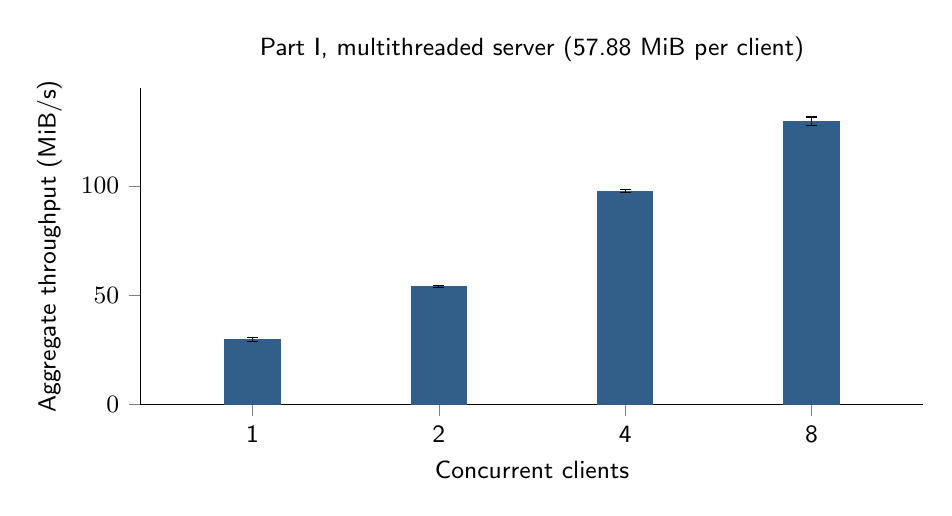
\begin{tikzpicture}
\begin{axis}[reportaxis,ybar,bar width=20pt,xlabel={Concurrent clients},ylabel={Aggregate throughput (MiB/s)},title={Part I, multithreaded server (57.88 MiB per client)},xtick={1,2,3,4},xticklabels={1,2,4,8},error bars/y dir=both,error bars/y explicit]
% BEGIN AUTO:part1plot
\addplot+[fill=barblue,draw=barblue,error bars/error bar style={black}] coordinates {(1,29.74671293) +- (0,0.81227542) (2,54.18542376) +- (0,0.44766272) (3,97.61279715) +- (0,0.58382875) (4,129.58119537) +- (0,1.98136043)};
% END AUTO:part1plot
\end{axis}\end{tikzpicture}\end{center}
\figurecaption{Aggregate throughput of the multithreaded server; error bars show sample standard deviation over three runs.}

\nextpage
% ======================== PAGE 5 ========================
\subsection{Analysis}
The multithreaded server averaged 29.75 MiB/s with one client and 129.58 MiB/s with eight. Single-threaded means were 30.13 and 29.27 MiB/s, respectively. At eight clients, the ratio of multithreaded to single-threaded mean throughput was 4.43. All clients requested the same complete image topic.

The host shares CPU, filesystem and memory resources between the server and clients. Small image files incur a manifest, file header, data ACK and file-transition exchange; this workload differs from a single large-file transfer. Variation across the three repetitions is shown by the error bars. These observations do not establish the throughput of a physical network link.

Without failed payload, payload send rate equals useful throughput. Application control overhead was 1,352,050 bytes for one client and 10,816,400 bytes for eight. The counters include both directions and cover framing, manifests and ACKs. Throughput and overhead graphs are included in \code{Results/Animals10/figures/}.

\section{Part II: fault-tolerant file transfer}
Part II builds on the multithreaded server, with one thread per active connection in every case. The server takes the third required argument, \code{failure_probability}, and deliberately drops connections. The cases differ in how they recover after a drop.

\subsection{Fault injection}
The failure decision is made after each DATA chunk has been sent and its ACK has been received. The serving thread draws a value in $[0,1)$ from \code{std::mt19937_64}; if it is below $p$, the server closes that connection. Each connection has its own stream, derived from a startup seed and its connection number. An optional seed supports repeatable stream generation, although concurrent connection ordering can vary.

The same decision point and 64 KiB chunk limit apply in all Part II cases. The draw can happen after the last data chunk of a file, before FILE\_END. A probability of zero disables injection. Values outside $[0,1]$ are rejected. Empty files and empty topics have no DATA decision point. Controlled proxy tests separately exercise failures during headers, within DATA, and at terminal messages.

The topic has 4,863 DATA chunks. One restart attempt succeeds with probability $(1-p)^M$. At $p=0.0003084$, this is approximately 0.2231, implying about 4.48 attempts under independent trials. The six rates were declared before measurement: 0.0000000, 0.00003084, 0.0000771, 0.0001542, 0.0002313, 0.0003084. They are identical across cases and scaled for the full topic. At $p=1$, a nonempty restart transfer cannot finish.

For result analysis, let $U$ be useful bytes, $T$ total file payload sent over every attempt, $A$ all application bytes sent in both directions, and $t$ batch time. Redundant payload is $T-U$, application control overhead is $A-T$, and useful throughput is $U/(t\,2^{20})$ MiB/s. Sent bytes are bytes accepted by socket send calls. These counters do not include Ethernet/IP/TCP headers or kernel TCP retransmissions.

\nextpage
% ======================== PAGE 6 ========================
\subsection{Case 1: no session management}
\subsubsection{Design}
Case 1 keeps no transfer checkpoint between attempts. The server is the Part I multithreaded service with fault injection and the same GET, OK, START, FILE\_HDR, DATA and completion exchanges. Every new connection requests a fresh transfer.

The client wraps the request in a retry loop, with 1,000 attempts by default. On reconnect it resets its cursor to the first file, validates the manifest and removes previously downloaded files belonging to that manifest before sending START. Thus an interruption in a late file causes earlier completed files to be transferred again. Retry delay starts at 5 ms and increases by 5 ms per attempt up to 100 ms. Measurement counters include work from failed attempts.

\subsubsection{Results}
\tablecaption{Case 1 on cane at $p=0.0003084$ (means of three completed runs)}
{\small\begin{tabularx}{\linewidth}{|Y|R|}\hline
\hdr Measure & \bfseries Value\rowend
% BEGIN AUTO:case1detail
Attempts & 4.33\rowend
Injected failures & 3.33\rowend
Useful payload & 60,686,716 bytes\rowend
Total payload sent & 132,898,224 bytes\rowend
Redundant payload & 72,211,508 bytes\rowend
Application control overhead & 3,453,659.33 bytes\rowend
Redundant share of sent payload & 54.34\%\rowend
Bytes sent per useful byte & 2.19\rowend
Completion time & 4.0822 s\rowend
Useful throughput & 17.49 MiB/s\rowend
% END AUTO:case1detail
\end{tabularx}}

\begin{center}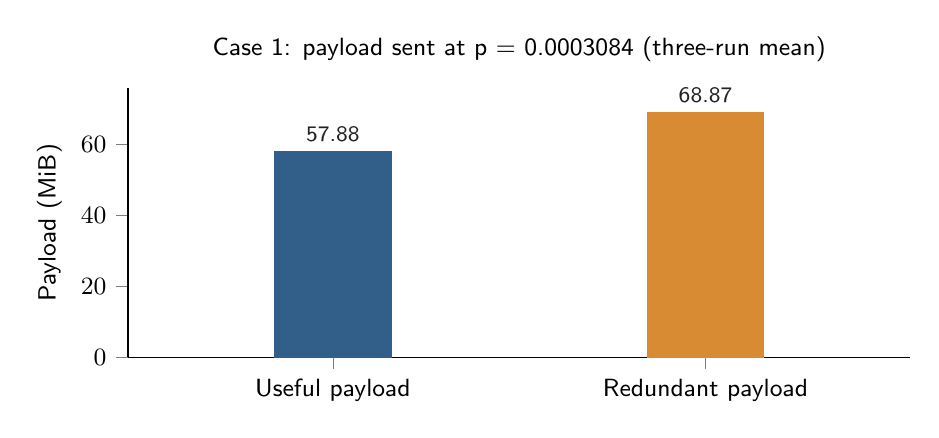
\begin{tikzpicture}
\begin{axis}[reportaxis,ybar,bar shift=0pt,bar width=42pt,height=50mm,xtick={1,2},xticklabels={Useful payload,Redundant payload},ylabel={Payload (MiB)},enlarge x limits=0.55,title={Case 1: payload sent at p = 0.0003084 (three-run mean)},nodes near coords,point meta=explicit symbolic,every node near coord/.append style={font=\footnotesize,text=bodytext}]
% BEGIN AUTO:case1plot
\addplot+[fill=barblue,draw=barblue] coordinates {(1,57.87536240) [57.88]};
\addplot+[fill=barorange,draw=barorange] coordinates {(2,68.86626085) [68.87]};
% END AUTO:case1plot
\end{axis}\end{tikzpicture}\end{center}
\figurecaption{Useful and redundant payload sent by the Case 1 server.}

\nextpage
% ======================== PAGE 7 ========================
\subsubsection{Analysis}
At $p=0.0003084$, Case 1 sent a mean 132,898,224.33 payload bytes to deliver 60,686,716 useful bytes. Redundant payload was 72,211,508.33 bytes, or 118.99\% of useful payload and 54.34\% of total sent payload. The transfer sent about 2.19 bytes per useful byte. These percentages use different denominators.

Mean completion time was 4.0822 s with injection at this rate and 1.9812 s with injection disabled. At $p=0.0002313$, mean injected failures were 2.33, mean completion time was 3.6270 s and redundant payload was 91.70\% of useful payload. Times include repeat work, setup and retry delays.

The raw logs retain every measured configuration, including low-failure runs. A finite random sample need not produce a strictly monotonic timing curve. The largest probability was selected from topic length before execution; it was not chosen after inspecting throughput. Fault counts, repeated bytes and elapsed time must be considered together when interpreting restart cost.

\subsection{Case 2: session management with checkpoint and resume}
\subsubsection{Design}
\tablecaption{Case 2 checkpoint-related messages}
{\small\begin{tabularx}{\linewidth}{|P{23mm}|P{42mm}|Y|}\hline
\hdr Direction & \bfseries Message & \bfseries Meaning\rowend
Client to server & GET with session ID & Starts a session or resumes the existing topic/worker assignment at a file-index and byte-offset cursor.\rowend
Server to client & OK, then FILE\_HDR & Returns the manifest and starts the expected file at the validated offset.\rowend
Server to client & DATA & Carries the next chunk and its CRC32. The server records the offered successor before sending.\rowend
Client to server & ACK & Confirms the client's cursor after recording a complete chunk or completing a file.\rowend
Server to client & FILE\_END, TRANSFER\_END & Completes a file or the worker's transfer. FILE\_END has its own ACK.\rowend
Server to client & ERROR & Rejects an unknown topic, mismatched assignment or invalid checkpoint; BUSY is retried.\rowend
\end{tabularx}}

\textbf{Client checkpoint.} The checkpoint is an in-memory record containing the session ID, topic, worker assignment, file index and byte offset. The client advances it only after a complete DATA frame passes CRC32 and its bytes are written successfully with \code{pwrite}. It then sends ACK. Unlike a durable checkpoint file, this record survives a dropped connection but not a restart of the client process.

\nextpage
% ======================== PAGE 8 ========================
\textbf{Server validation.} The server maintains a mutex-protected table of session records. Each record stores the topic and worker assignment, a committed cursor and the last offered successor. On reconnect, the client reports its session ID and cursor. Only the committed cursor or that exact offered successor is accepted. An arbitrary offset, wrong assignment or expired noninitial session is rejected.

This distinction handles a lost ACK. If the client wrote a chunk but its ACK disappeared, its cursor is the offered successor and the server can commit it during reconnection. If the connection broke in the middle of a frame, the client still reports the committed cursor and the incomplete chunk is sent again. Only uncommitted data may need retransmission.

\textbf{File boundaries.} FILE\_END is acknowledged with the next assigned file index, including for empty files. A loss of FILE\_END, its ACK or TRANSFER\_END is recoverable. On reopening an interrupted file, the client truncates any uncommitted tail. Server sessions remain in memory, with 600-second idle retention and a 10,000-record limit; neither endpoint provides process-crash recovery.

\subsubsection{Results}
\tablecaption{Case 2 on cane (60,686,716 useful bytes, three runs per probability)}
{\small\begin{tabularx}{\linewidth}{|R|R|R|R|R|R|}\hline
\hdr $p\, (10^{-4})$ & \bfseries Injected failures & \bfseries Redundant bytes & \bfseries Control bytes & \bfseries Time (s) & \bfseries MiB/s\rowend
% BEGIN AUTO:case2results
0.000 & 0.00 & 0 & 1,352,050 & 1.9355 & 29.93\rowend
2.313 & 1.33 & 0 & 1,657,047 & 2.0373 & 28.41\rowend
3.084 & 1.33 & 0 & 1,657,047 & 2.0480 & 28.27\rowend
% END AUTO:case2results
\end{tabularx}}

\begin{center}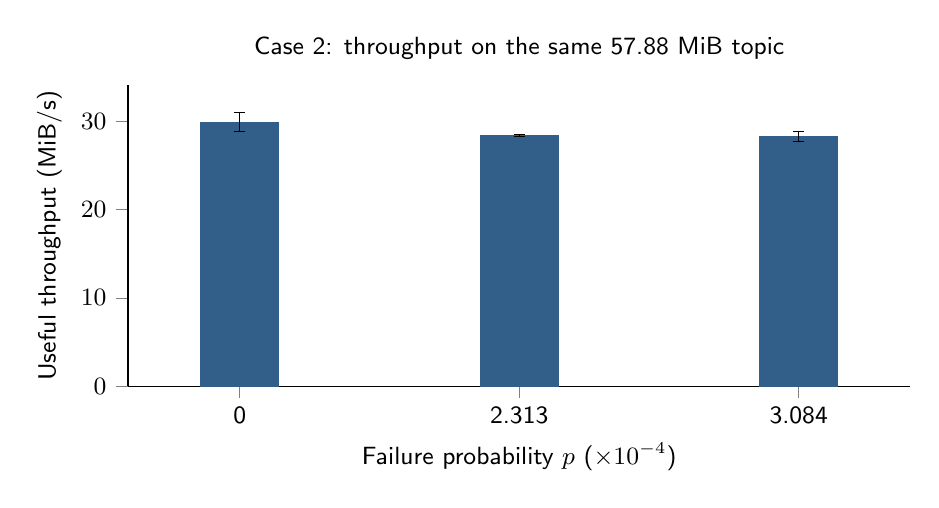
\begin{tikzpicture}
\begin{axis}[reportaxis,ybar,bar width=28pt,height=54mm,xtick={1,2,3},xticklabels={0,2.313,3.084},xlabel={Failure probability $p$ ($\times 10^{-4}$)},ylabel={Useful throughput (MiB/s)},title={Case 2: throughput on the same 57.88 MiB topic},error bars/y dir=both,error bars/y explicit]
% BEGIN AUTO:case2plot
\addplot+[fill=barblue,draw=barblue,error bars/error bar style={black}] coordinates {(1,29.92711047) +- (0,1.06415589) (2,28.40776928) +- (0,0.10636730) (3,28.26672642) +- (0,0.58372912)};
% END AUTO:case2plot
\end{axis}\end{tikzpicture}\end{center}
\figurecaption{Case 2 throughput; error bars show sample standard deviation. Mean failure counts are listed in Table 6.}

\nextpage
% ======================== PAGE 9 ========================
Every completed benchmark download matched all 4,863 source SHA-256 values. Under the built-in post-ACK fault policy, Case 2 sent exactly 60,686,716 payload bytes at every measured probability. Separate integration checks cover lost DATA ACKs and recovery of incomplete frames; all 28 checks passed. The integration logs are in \code{Results/Validation/}.

\tablecaption{Case 1 and Case 2 on the same topic at the same $p=0.0003084$ (three-run means)}
{\small\begin{tabularx}{\linewidth}{|Y|R|R|}\hline
\hdr Measure & \bfseries Case 1 & \bfseries Case 2\rowend
% BEGIN AUTO:casecomparison
Attempts & 4.33 & 2.33\rowend
Payload sent (bytes) & 132898224 & 60686716\rowend
Redundant bytes & 72211508 & 0\rowend
Application control bytes & 3453659.33 & 1657047.33\rowend
Completion time (s) & 4.0822 & 2.0480\rowend
Useful throughput (MiB/s) & 17.49 & 28.27\rowend
% END AUTO:casecomparison
\end{tabularx}}

\begin{center}
\begin{minipage}{0.48\linewidth}\centering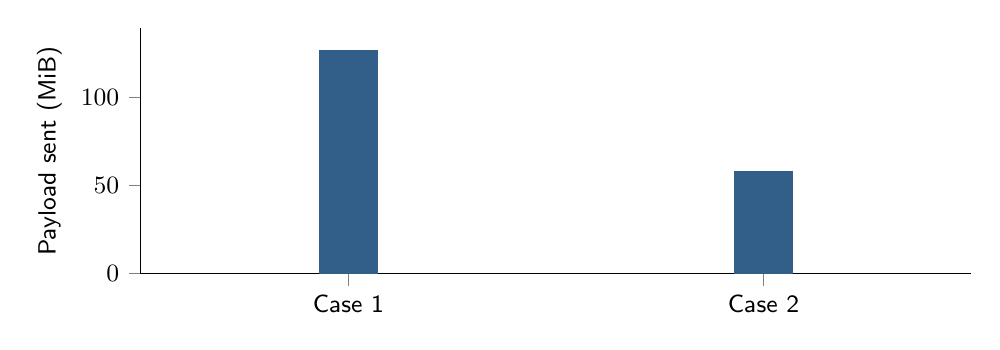
\begin{tikzpicture}
\begin{axis}[reportaxis,width=\linewidth,height=47mm,ybar,bar width=21pt,xtick={1,2},xticklabels={Case 1,Case 2},ylabel={Payload sent (MiB)},enlarge x limits=.5]
% BEGIN AUTO:comparisonbytes
\addplot+[fill=barblue,draw=barblue] coordinates {(1,126.74162324) (2,57.87536240)};
% END AUTO:comparisonbytes
\end{axis}\end{tikzpicture}\end{minipage}\hfill
\begin{minipage}{0.48\linewidth}\centering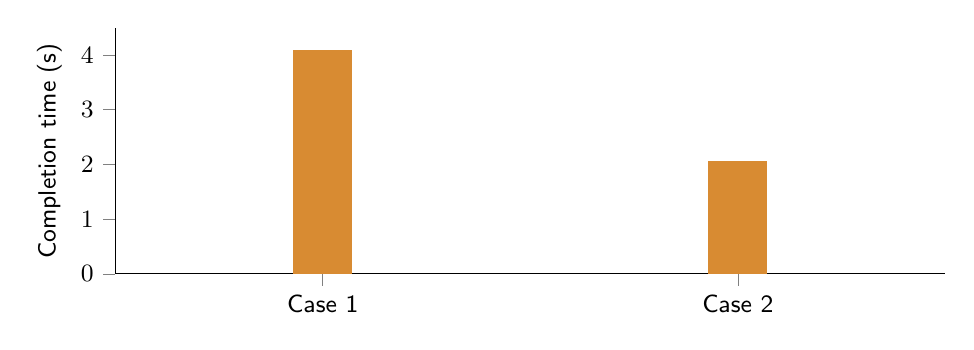
\begin{tikzpicture}
\begin{axis}[reportaxis,width=\linewidth,height=47mm,ybar,bar width=21pt,xtick={1,2},xticklabels={Case 1,Case 2},ylabel={Completion time (s)},enlarge x limits=.5]
% BEGIN AUTO:comparisontime
\addplot+[fill=barorange,draw=barorange] coordinates {(1,4.08216795) (2,2.04804853)};
% END AUTO:comparisontime
\end{axis}\end{tikzpicture}\end{minipage}
\end{center}
\figurecaption{Payload sent and completion time for restart and resume on cane, at $p=0.0003084$.}

\subsubsection{Analysis}
At $p=0.0003084$, Case 2 completed in a mean 2.0480 s versus 4.0822 s for Case 1; the ratio of mean times was 1.99. Mean useful throughput was 28.27 and 17.49 MiB/s, respectively. Checkpoints avoided repeating recorded file data under this injection policy; reconnects, manifests, ACKs and retry pauses still incurred costs.

The no-redundancy result depends on injection occurring after ACK. A break during a frame may require an uncommitted chunk to be repeated. Clean Case 2 averaged 29.93 MiB/s, compared with 29.75 MiB/s for Part I multi mode with one client. Both use the same Animals10 topic, but three shared-host repetitions do not isolate a precise checkpoint-management cost.

\nextpage
% ======================== PAGE 10 ========================
\subsection{Case 2 Enhanced: parallel connections}
\subsubsection{Design}
The main enhancement is parallel TCP connections: one logical client opens $K$ connections for a topic and runs a worker thread on each. The default is four, with an optional client argument allowing one to 32. Blocking sockets are retained on both endpoints. A worker blocked in \code{send} or \code{recv} holds up its own connection, while the other workers can continue.

\tablecaption{Case 2 Enhanced messages}
{\small\begin{tabularx}{\linewidth}{|P{23mm}|P{42mm}|Y|}\hline
\hdr Direction & \bfseries Message & \bfseries Meaning\rowend
Client to server & GET(topic, worker, $K$, cursor) & Opens or resumes this worker's session. The frame carries its independent session ID.\rowend
Server to client & OK(manifest) & Sends the complete ordered manifest. Assignment is determined from file index and worker count.\rowend
Client to server & START & Requests the files assigned to this worker.\rowend
Server to client & FILE\_HDR and DATA & Sends only this worker's files, from the validated cursor.\rowend
Client to server & ACK(cursor) & Commits a written chunk or file transition in this worker's session.\rowend
Server to client & FILE\_END, TRANSFER\_END & Completes a file or all work assigned to this worker.\rowend
Server to client & ERROR & Rejects an inconsistent assignment or checkpoint; BUSY can be retried.\rowend
\end{tabularx}}

\textbf{Splitting the work.} The server sorts the topic files and assigns file index $i$ to worker $i\bmod K$. With $K=4$, worker 0 receives indices 0, 4, 8 and so on. Splitting by whole files gives each file exactly one writer. Reassembly is simply writing each assigned file under its own name; there is no shared-file byte-range merge.

\textbf{Recovery.} Every worker keeps its own in-memory checkpoint and session ID. On a drop, only that worker reconnects and reports its cursor. The server verifies the topic, worker, count and committed/offered state using the Case 2 protocol. Other workers continue. The main client joins all workers and reports success only if every worker finishes.

\textbf{Trade-offs.} Each connection receives a full manifest and requires a socket, thread and session. File-level assignment can be uneven if file sizes vary. A topic with only one file cannot exploit several workers. If $K$ exceeds the number of files, idle workers perform only their manifest and completion exchange. A dynamic file queue or byte-range splitting could improve load balance but is not implemented.

Both the server session table and worker checkpoints are volatile. Connection failures are recoverable; process restarts and power loss are outside the implemented guarantee. Output writes are not fsynced after every chunk.

\nextpage
% ======================== PAGE 11 ========================
\subsubsection{Results}
\tablecaption{Case 2 Enhanced on cane with four workers (three-run means)}
{\small\begin{tabularx}{\linewidth}{|R|R|C|R|R|}\hline
\hdr $p\, (10^{-4})$ & \bfseries Injected failures & \bfseries Control bytes & \bfseries Time (s) & \bfseries MiB/s\rowend
% BEGIN AUTO:enhancedresults
0.000 & 0.00 & 2,038,153 & 0.8781 & 66.10\rowend
2.313 & 1.33 & 2,343,150 & 0.8199 & 70.93\rowend
3.084 & 2.00 & 2,495,649 & 0.9060 & 63.96\rowend
% END AUTO:enhancedresults
\end{tabularx}}

Each run delivered all 4,863 images and every SHA-256 matched. With four workers, file counts were 1,216, 1,216, 1,216 and 1,215. Assigned bytes ranged from 14.40 to 14.66 MiB because image sizes differ. No payload was repeated under post-ACK injection. Full sweeps and overhead graphs are in \code{Results/Animals10/}.

Connection count was also measured at $p=0.0000771$. Mean throughput was 26.60, 45.48, 71.12, 69.11 MiB/s for $K=1,2,4,8$. Corresponding mean completion times were 2.1797, 1.2985, 0.8177, 0.8383 s.

\begin{center}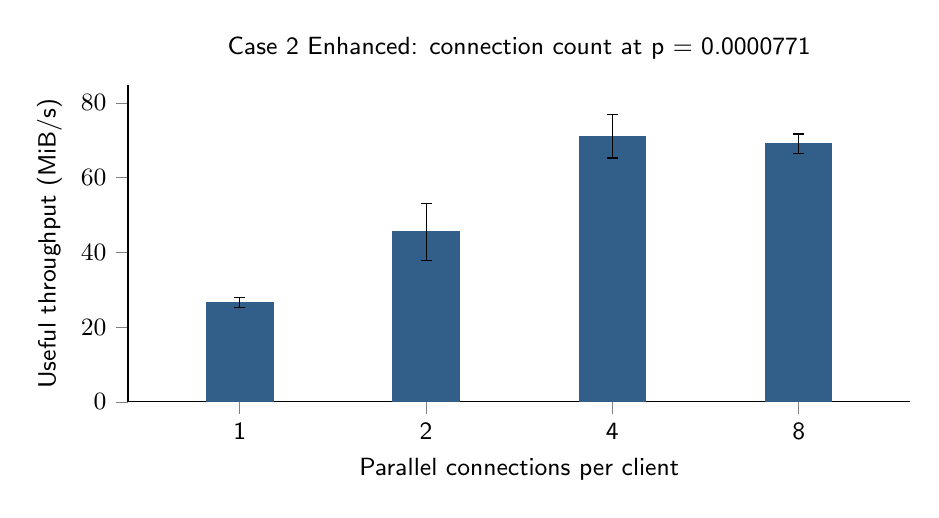
\begin{tikzpicture}
\begin{axis}[reportaxis,ybar,bar width=24pt,height=56mm,xtick={1,2,3,4},xticklabels={1,2,4,8},xlabel={Parallel connections per client},ylabel={Useful throughput (MiB/s)},title={Case 2 Enhanced: connection count at p = 0.0000771},error bars/y dir=both,error bars/y explicit]
% BEGIN AUTO:enhancedplot
\addplot+[fill=barblue,draw=barblue,error bars/error bar style={black}] coordinates {(1,26.60292356) +- (0,1.41653722) (2,45.47846072) +- (0,7.61529043) (3,71.11630266) +- (0,5.86811192) (4,69.10573113) +- (0,2.57340993)};
% END AUTO:enhancedplot
\end{axis}\end{tikzpicture}\end{center}
\figurecaption{Measured enhanced throughput versus connection count; error bars show sample standard deviation.}

\subsubsection{Analysis}
The ratio of eight-connection to one-connection mean throughput was 2.60 for this image topic. Workers can overlap socket waits, CRC checks and file operations, while CPU and storage remain shared. Each worker owns whole files, so uneven sizes and filesystem contention can limit scaling. The observed ratio is specific to this dataset and host.

Four-worker mean throughput was 63.96 MiB/s at $p=0.0003084$ and 66.10 MiB/s without injection. Nonmonotonic differences, where present, can reflect sampling and scheduling; they are not evidence that faults improve performance. Clean four-worker control traffic was 2,038,153 bytes, compared with 1,352,050 for one worker, because each connection receives a complete manifest.

\nextpage
% ======================== PAGE 12 ========================
\section{Summary of observations}
\tablecaption{The implementations side by side}
{\small\begin{tabularx}{\linewidth}{|P{28mm}|P{25mm}|P{38mm}|Y|}\hline
\hdr Implementation & \bfseries After a failure & \bfseries State kept & \bfseries Main measured result\rowend
Part I, single-threaded & No recovery & No retained transfer checkpoint & 27.91--30.13 MiB/s across 1, 2, 4 and 8 clients.\rowend
Part I, multithreaded & No recovery & No retained transfer checkpoint & 29.75 and 129.58 MiB/s with 1 and 8 clients.\rowend
Case 1 & Restart the topic & No recovery state & 4.33 mean attempts; 118.99\% extra payload at the highest $p$.\rowend
Case 2 & Resume at cursor & Client cursor; server committed/offered session state & Zero repeated payload under injection; 2.0480 s at the highest $p$.\rowend
Case 2 Enhanced & Resume each worker & Independent client cursors and server sessions & Four workers: 63.96 MiB/s at the highest $p$; all images verified.\rowend
\end{tabularx}}

The experiments compare sequential and concurrent service, full restart and checkpoint recovery, and different connection counts on one complete Animals10 topic. Restart recovery repeats completed work; checkpoint recovery avoids repeating recorded chunks under the implemented fault policy. Parallel execution changes throughput and control costs. The raw observations and all graphs are supplied for independent inspection.

\section{Deviations from the design and limitations}
\begin{itemize}
\item The submitted design is implemented using C++17 containers with POSIX sockets and pthreads. Binary framing and a GET carrying the existing session ID implement the conceptual messages and RESUME operation. The protocol and report describe the actual code.
\item All report measurements use the real Animals10 images on one Linux host. The required experiment with one server computer and two client computers remains unperformed. Local TCP processes do not satisfy that topology requirement; LAN scripts are included.
\item Each configuration has three repetitions. The host is shared and page cache is not controlled. Reported means and sample deviations do not establish physical-network performance or a universal speed-up.
\item Checkpoints are in memory. Process restart, power loss, changing source files, authenticated access and encrypted transport are not provided. CRC32 detects accidental chunk errors; it is not an authentication mechanism.
\item All 28 integration checks passed, and a Case 2 ASan/UBSan recovery smoke run reported no error. LeakSanitizer was disabled because the sandbox restricts process inspection. These checks are evidence of tested behavior, not a proof that no bug exists.
\end{itemize}
{\footnotesize\color{muted}\textbf{Preparation note.} The supplied Group 065/083 report is credited as the layout and organizational reference. Technical descriptions and results here correspond to the Group 097/112 implementation and logs. The package was prepared with AI assistance; the group should review the work and confirm actual contributions before submission.}
\end{document}
